%% The following is a directive for TeXShop to indicate the main file
%%!TEX root = diss.tex

\chapter{Particle Identification}
\label{ch:Results}
%\section{Particle Identification}
\label{sec:particleIdentification}
In order to identify particles using the \ac{ARICH} detector, a particle likelihood method is used \cite{richImpact, belleArich}.
For this method, we take the measured momentum of the particle, and determined the expected velocity for different candidate particles masses.
The candidate particles of interest for this study are protons, with a mass of 0.938 GeV/c$^2$, pions, with a mass of 0.140 GeV/c$^2$, and kaons, with a mass of 0.494 GeV/c$^2$\TODO{cite pdg}.
To calculate the velocity, we then use the following relativistic equation, assuming units where $c = 1$:

\begin{equation}
\label{eq:relMass}
 \beta = \sqrt{\frac{1}{1 +m^2 / p^2}}
\end{equation}


For each velocity hypothesis, we run 10,000 simulations of particles moving at that velocity, with the same measured initial trajectory as the input event data, and get the distribution of the resulting photons.
For each pixel of the detector, this procedure will give a value $\lambda_i(\beta)$, equal to the expected number of photons striking pixel $i$ in the detector due to a particle of velocity $\beta$. 

For a given event, we will detect $N_i$ photons in each pixel $i$.
In reality, the PMTs are only capable of registering whether or not a photon has been detected - if multiple photons strike a single pixel in a very short amount of time, it will not be able to distinguish the number detected, so we just know if $N_i = 0$ or $N_i > 0$.

If we assume that the number of photons detected by a PMT pixel is given by a Poisson distribution, then the probability that zero photons strike pixel $i$ is given by:
\begin{equation}
P_i(N_i=0; \beta) = e^{-\lambda_i(\beta)}
\end{equation}

 The probability that one or more photons strike pixel $i$ must then be:
\begin{equation}
P_i(N_i>1; \beta) = 1 - e^{-\lambda_i(\beta)}
\end{equation}

By multiplying the probabilities of getting the observed result in each pixel $i$ of the detector, we calculate the likelihood for that value of $\beta$:

\begin{equation}
L_\beta = \prod_{i}P_i(N_i; \beta)
\end{equation}

Because of the floating point errors that would inevitably be introduced by multiplying hundreds of numbers together, we instead can look at twice the negative log of the likelihood:

\begin{equation}
    \label{eq:log-likelihood}
    -2\ln(L_\beta) = -2\sum_i \ln(P_i(N_i; \beta))
\end{equation}

Because the log function is montonic, maximizing the likelihood function is equivalent to minimizing the negative log-likelihood.
%One potential downside to using the negative log-likelihood is that if some bin has a computed value $\lambda$ of 0, then the likelihood of the distribution becomes $-\infinity$. 
%Because this may lead to numerical problems, we may apply some additive smoothing.
For each event, the negative log-likelihood can be calculated for each particle hypothesis, and we can predict that each event was caused by the particle that minimizes the negative log-likelihood.

The full code implementing this particle identification approach and the fast ARICH simulation is described in more detail in Appendix A.

\section{Particle Separation}
With this approach to particle identification in place, it is necessary to establish the effectiveness of the technique under different conditions.
As an example, let us suppose we want to determine how well this likelihood approach works on a particle that is 7 GeV and measured to enter the center of the aerogel and travel directly in the z-direction.
To check the certainty with which this technique can identify whether this is a pion or kaon, I applied the following procedure:

\begin{enumerate}
\item Generate 10,000 pions with the given position, direction, and momenta in Geant4, project the generated Cherenkov photons onto a plane representing the detector, apply efficiency corrections, and store the resulting histogram of detected photon hits for each pion. 
\item Do the same, but with simulated kaons instead of pions.
\item Given the particle initial position, initial direction, and momentum, use the fast ARICH simulation to generate two photon probability distribution histograms, corresponding to pions or kaons.
\item For each event simulated using Geant4, compute the negative log-likelihood of the event histogram with respect to the photon probability distribution functions of each particle hypothesis.
\item For each true particle type, plot a histogram of the log of the ratio of likelihoods between the two hypotheses.
This is just the differences between the negative log-likelihoods of the two hypotheses.
\item Look at the separation between the distributions: this is equal to the difference in means between the distributions, divided by the root mean square of each distribution added in quadrature
\end{enumerate}

The result of this procedure is shown in Figure \ref{fig:kaonpionsep}. The two distributions are separated by a distance of $2.4 \sigma$ - the significant overlap between the two distribution indicates that there is some chance of misidentification. Applying the same procedure to verify the separation between kaons and protons gives the results shown in Figure \ref{fig:kaonprotonsep}. Here we see that the two distributions do not significantly overlap and have a separation of $4.7 \sigma$, meaning that at this momentum and angle, protons are very unlikely to be misidentified as kaons, and vice versa.
\begin{figure}[]
\centering
\resizebox{0.9\textwidth}{!}{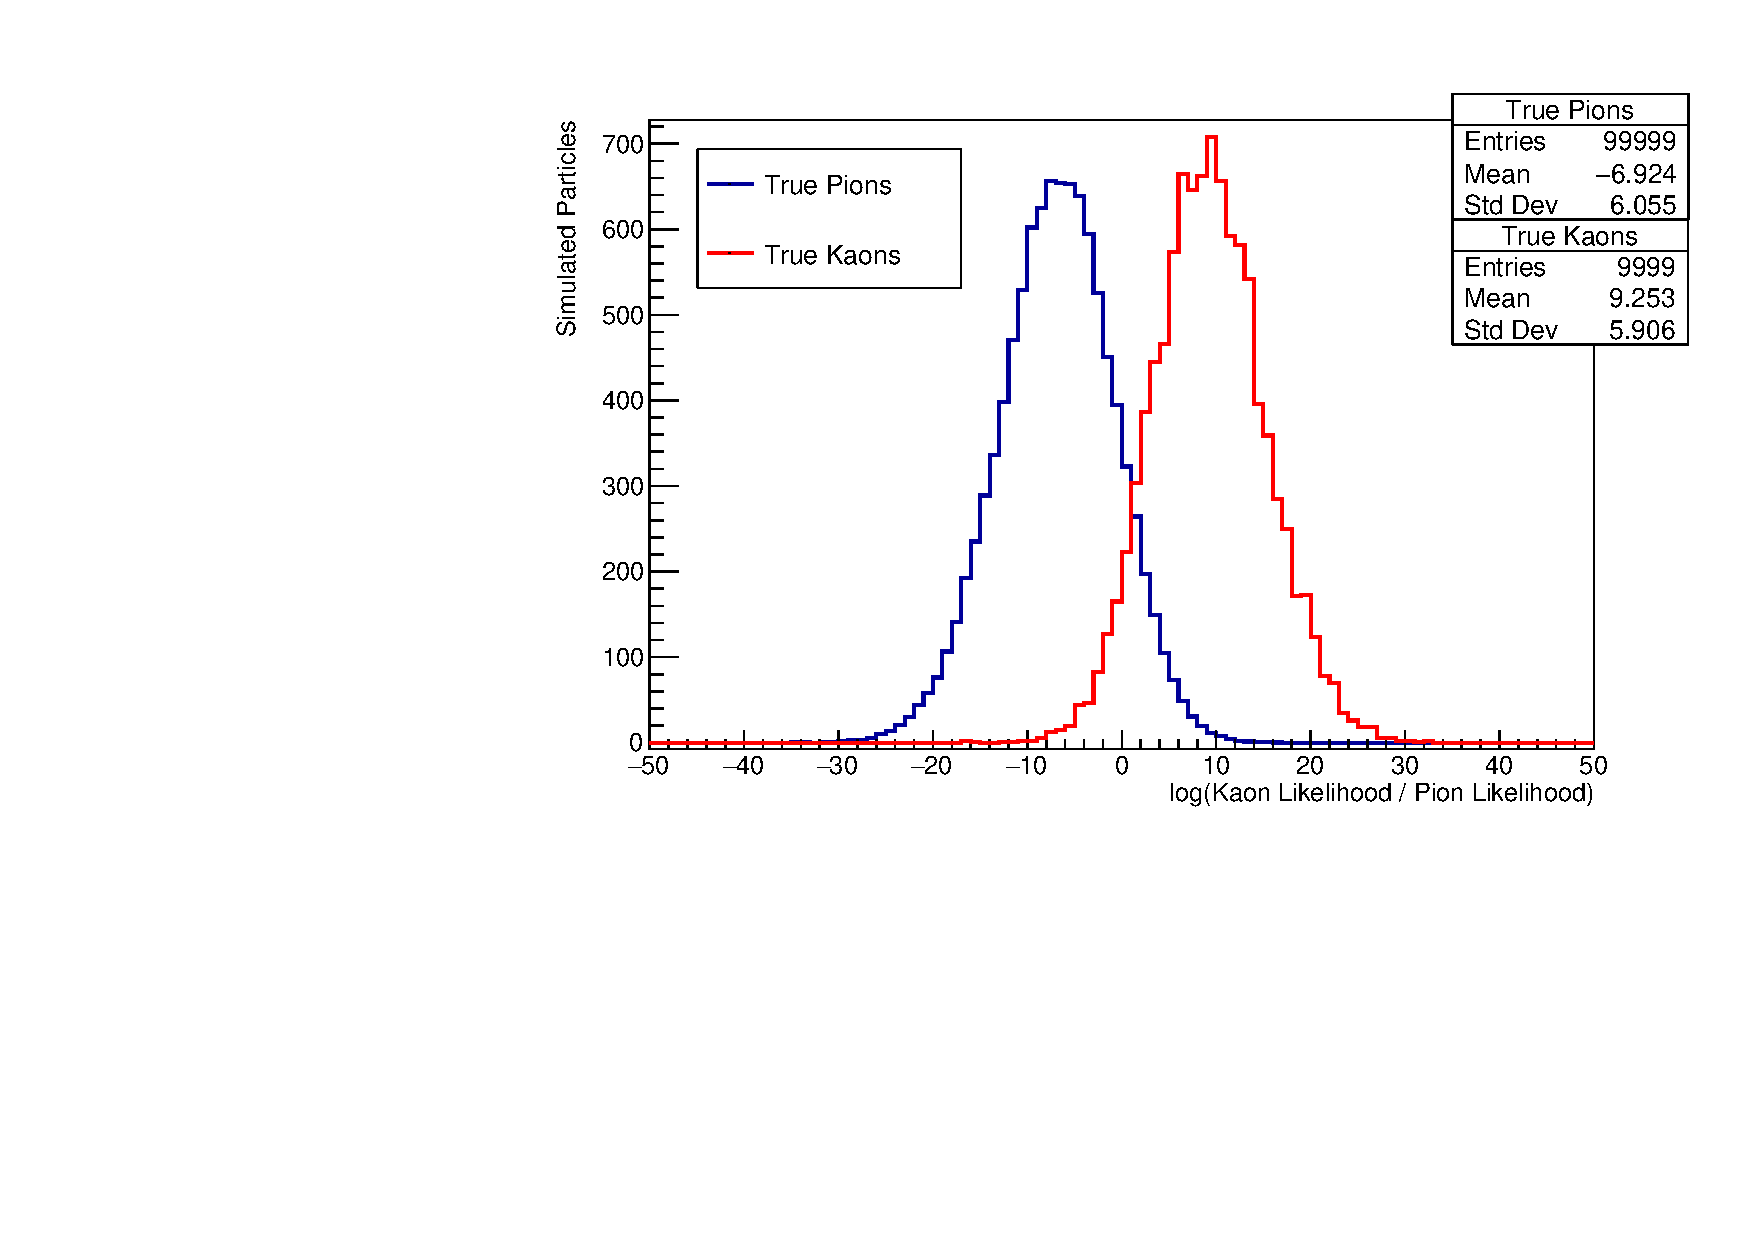
\includegraphics{./figs/kaonPionSep.pdf}}
\caption[Particle identification separation for 7 GeV pions and kaons]{Histogram showing the logarithm of the ratios of likelihoods between kaons and pions for both ``true" kaons and ``true" pions. The two distributions have a separation of 2.4 $\sigma$.}
\label{fig:kaonpionsep} 
\end{figure}

\begin{figure}[]
\centering
\resizebox{0.9\textwidth}{!}{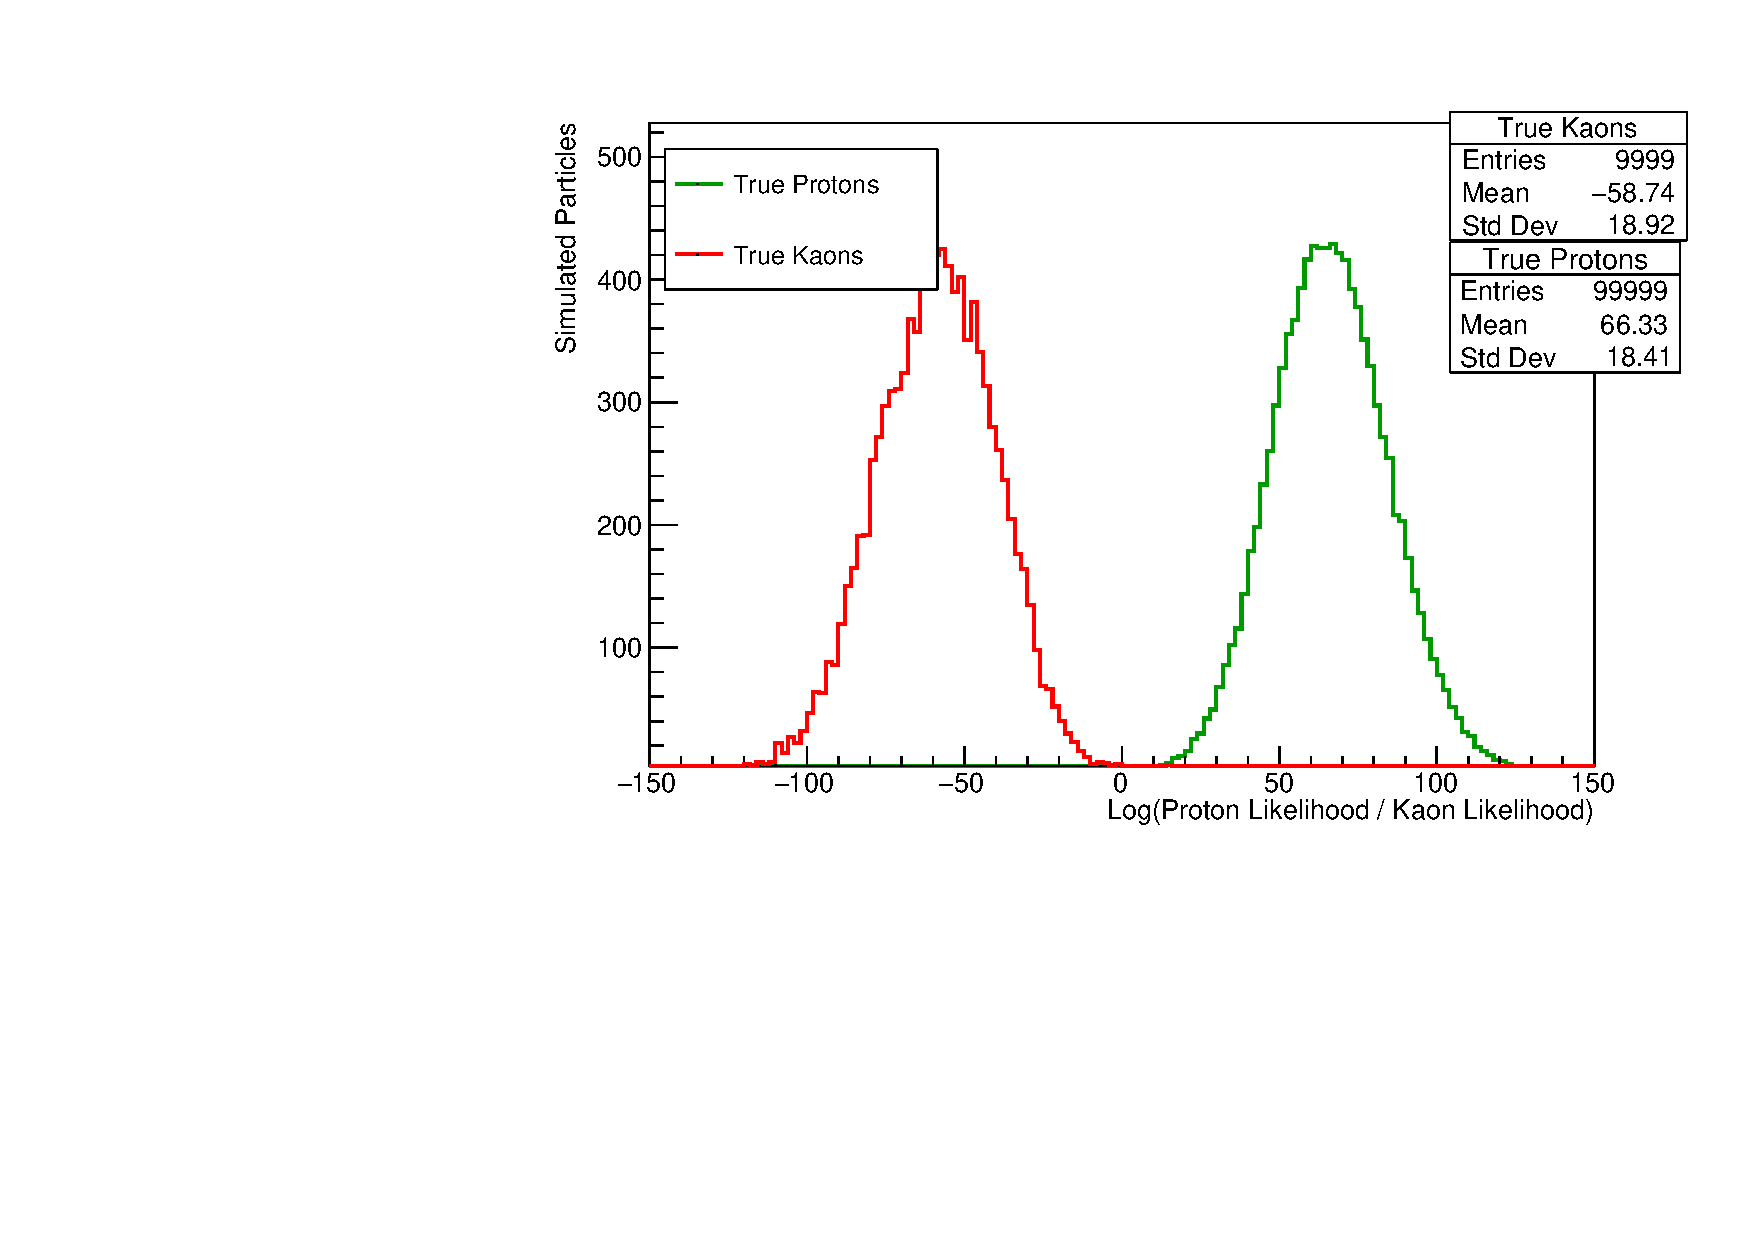
\includegraphics{./figs/kaonProtonSep.pdf}}
\caption[Particle identification separation for 7 GeV kaons and protons]{Histogram showing the logarithm of the ratios of likelihoods between protons and kaons for both ``true" protons and ``true" kaons. The two distributions have a separation of  4.7 $\sigma$.}
\label{fig:kaonprotonsep} 
\end{figure}

\subsection{Momenta}

Figure \ref{fig:changles} shows that at increasing momenta, it becomes increasingly hard to distinguish between particles, as their velocities converge to $c$ and their Cherenkov angles in a given aerogel converge to the same value.
It is particularly hard to distinguish between pions and kaons, but easier to distinguish protons from kaons, and easier still to distinguish protons from pions.

\begin{figure}[]
\centering
\resizebox{0.9\textwidth}{!}{\includegraphics{./figs/changles2.pdf}}
\caption[Predicted Cherenkov angles of pions, kaons, and protons over a range of momenta.]{Predicted Cherenkov angles of pions, kaons, and protons over a range of momenta.}
\label{fig:changles}
\end{figure}



A script was written to automate this procedure over a range of different initial particle directions and particle momenta. 
Figure \ref{fig:centeredSeps} shows the separation between likelihood distributions for each particle-particle pair over a range of momenta from 6 GeV/c to 14 GeV/c, with particles travelling directly down the $z$-axis.
The effectiveness of this technique for particle separation can also be measured by looking at misidentification rates: that is, the percentage of the time the particle identity that yielded the minimum negative log-likelihood among the candidate particles was not the true particle.
This is shown in Figure \ref{fig:centeredMis}.

\begin{figure}[]
\centering
\resizebox{0.9\textwidth}{!}{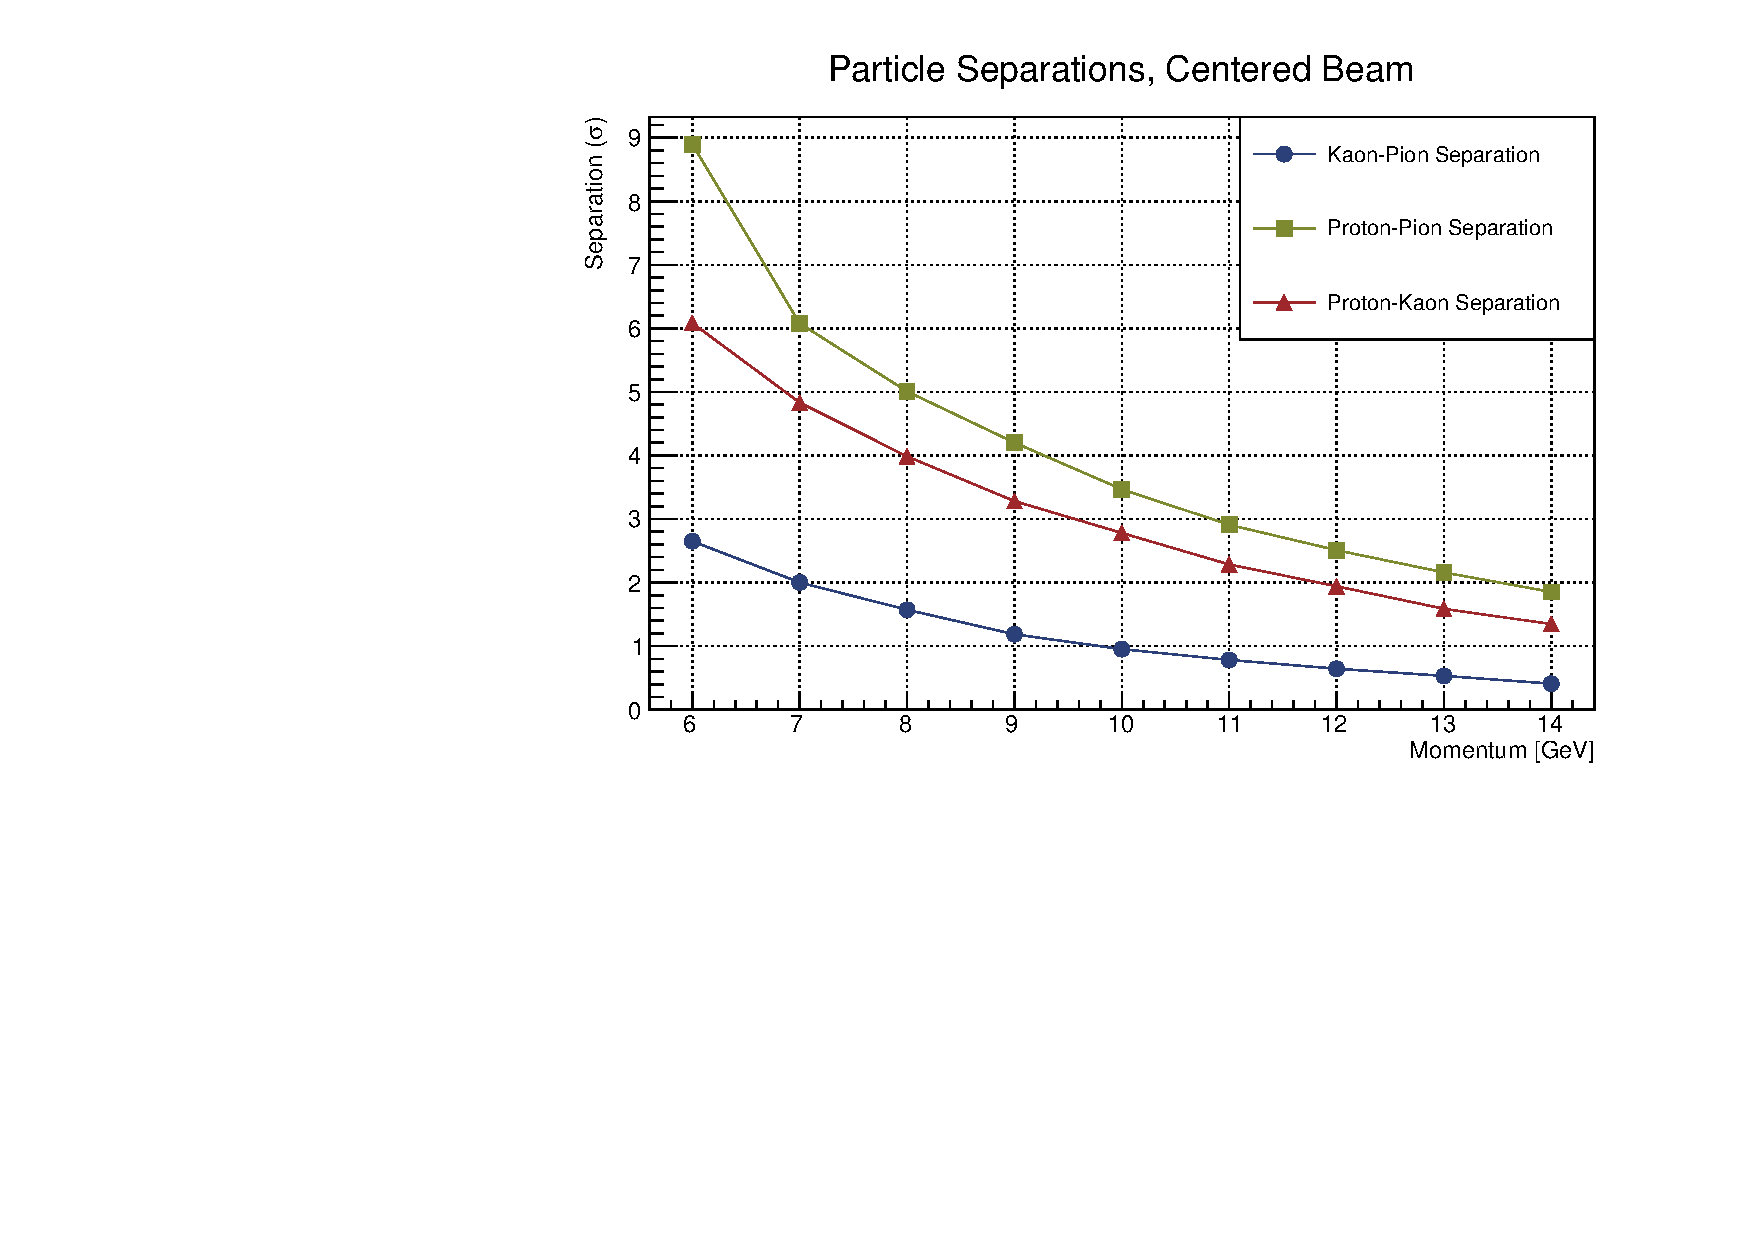
\includegraphics{./figs/centeredSeps.pdf}}
\caption[\TODO{}]{\TODO{Caption}}
\label{fig:centeredSeps} 
\end{figure}

\begin{figure}[]
\centering
\resizebox{0.9\textwidth}{!}{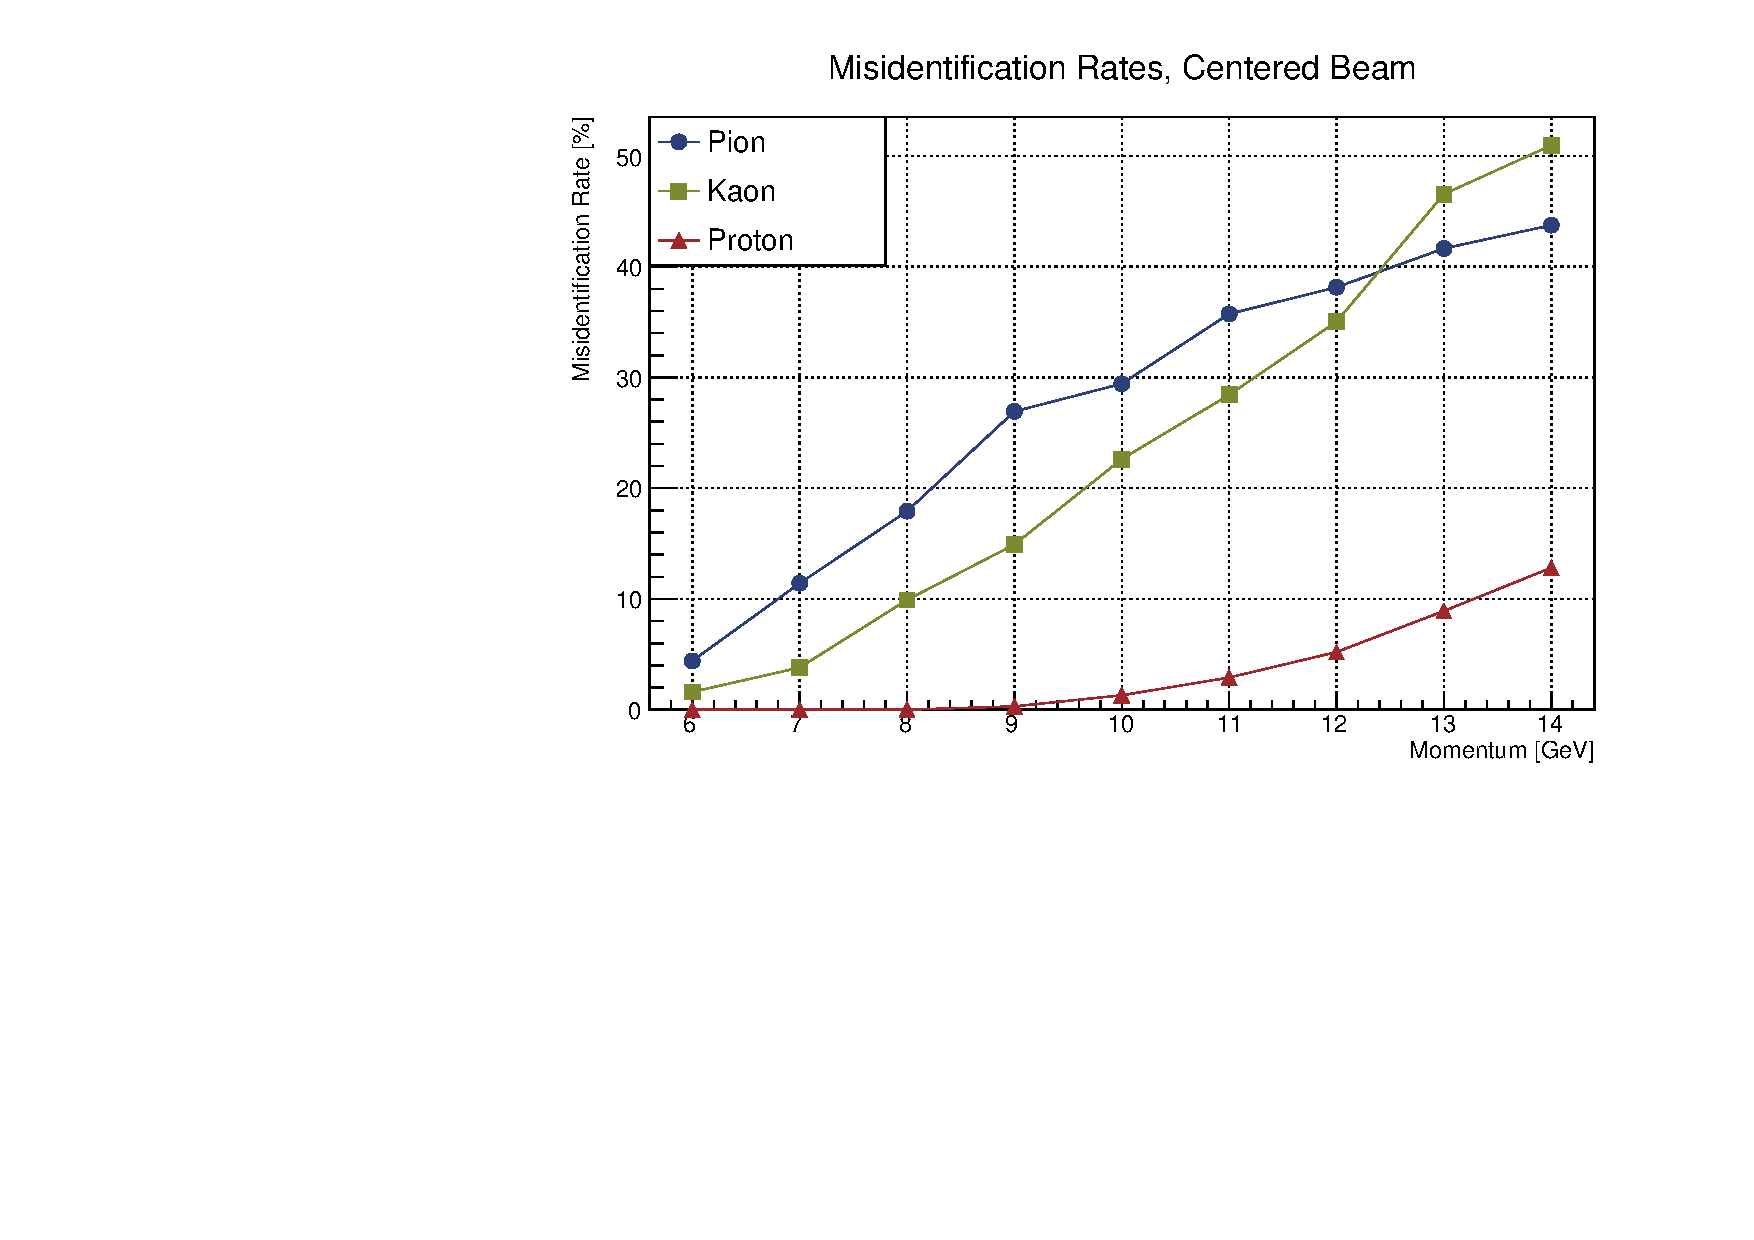
\includegraphics{./figs/centeredMisidentification.pdf}}
\caption[\TODO{}]{\TODO{Caption}}
\label{fig:centeredMis} 
\end{figure}

We see that as momentum increases, we steadily become worse and worse at distinguishing between pions and kaons - we get a separation greater than $2 \sigma$ past momenta of 7 GeV/c, and at a momentum of 14 GeV/c, we do no better than luck at determining whether a particle is a kaon or pion.
We see that it does not become difficult to distinguish between a proton and a pion or a proton and a kaon up until we reach approximately 12 or 13 GeV/c. 

\subsection{Angles}
When particles enter the aerogel at nonzero angles with respect to the beamline axis, a number of intractable effects affect the resulting photon distribution. 
Particles travel further through the aerogel at higher angles and may produce more photons, photons refract differently, and the resulting Cherenkov cones may become smeared out over more PMT pixels. 
To evaluate the effectiveness of this likelihood approach across different angles, the procedure described in the preceding section was followed over 5 angular bins ranging from 0 to 0.4 radians.
The resulting particle separations are shown in Figure \ref{fig:angleSeps}.

It is clear that as the angle of the incident particle increases, we become better able to separate out our particles from one another up until a certain point.
This is likely because the photon rings are ``smeared out" over several different PMT pixels, allowing for finer details to be measured. 
However, past 0.35 radians we see that our ability to distinguish particles significantly decreases.
This is because at this point, the photon rings partially fall off of the detector plane, and with fewer detected photons, there is less information to distinguish particles.

\begin{figure}[]
\centering
\resizebox{0.9\textwidth}{!}{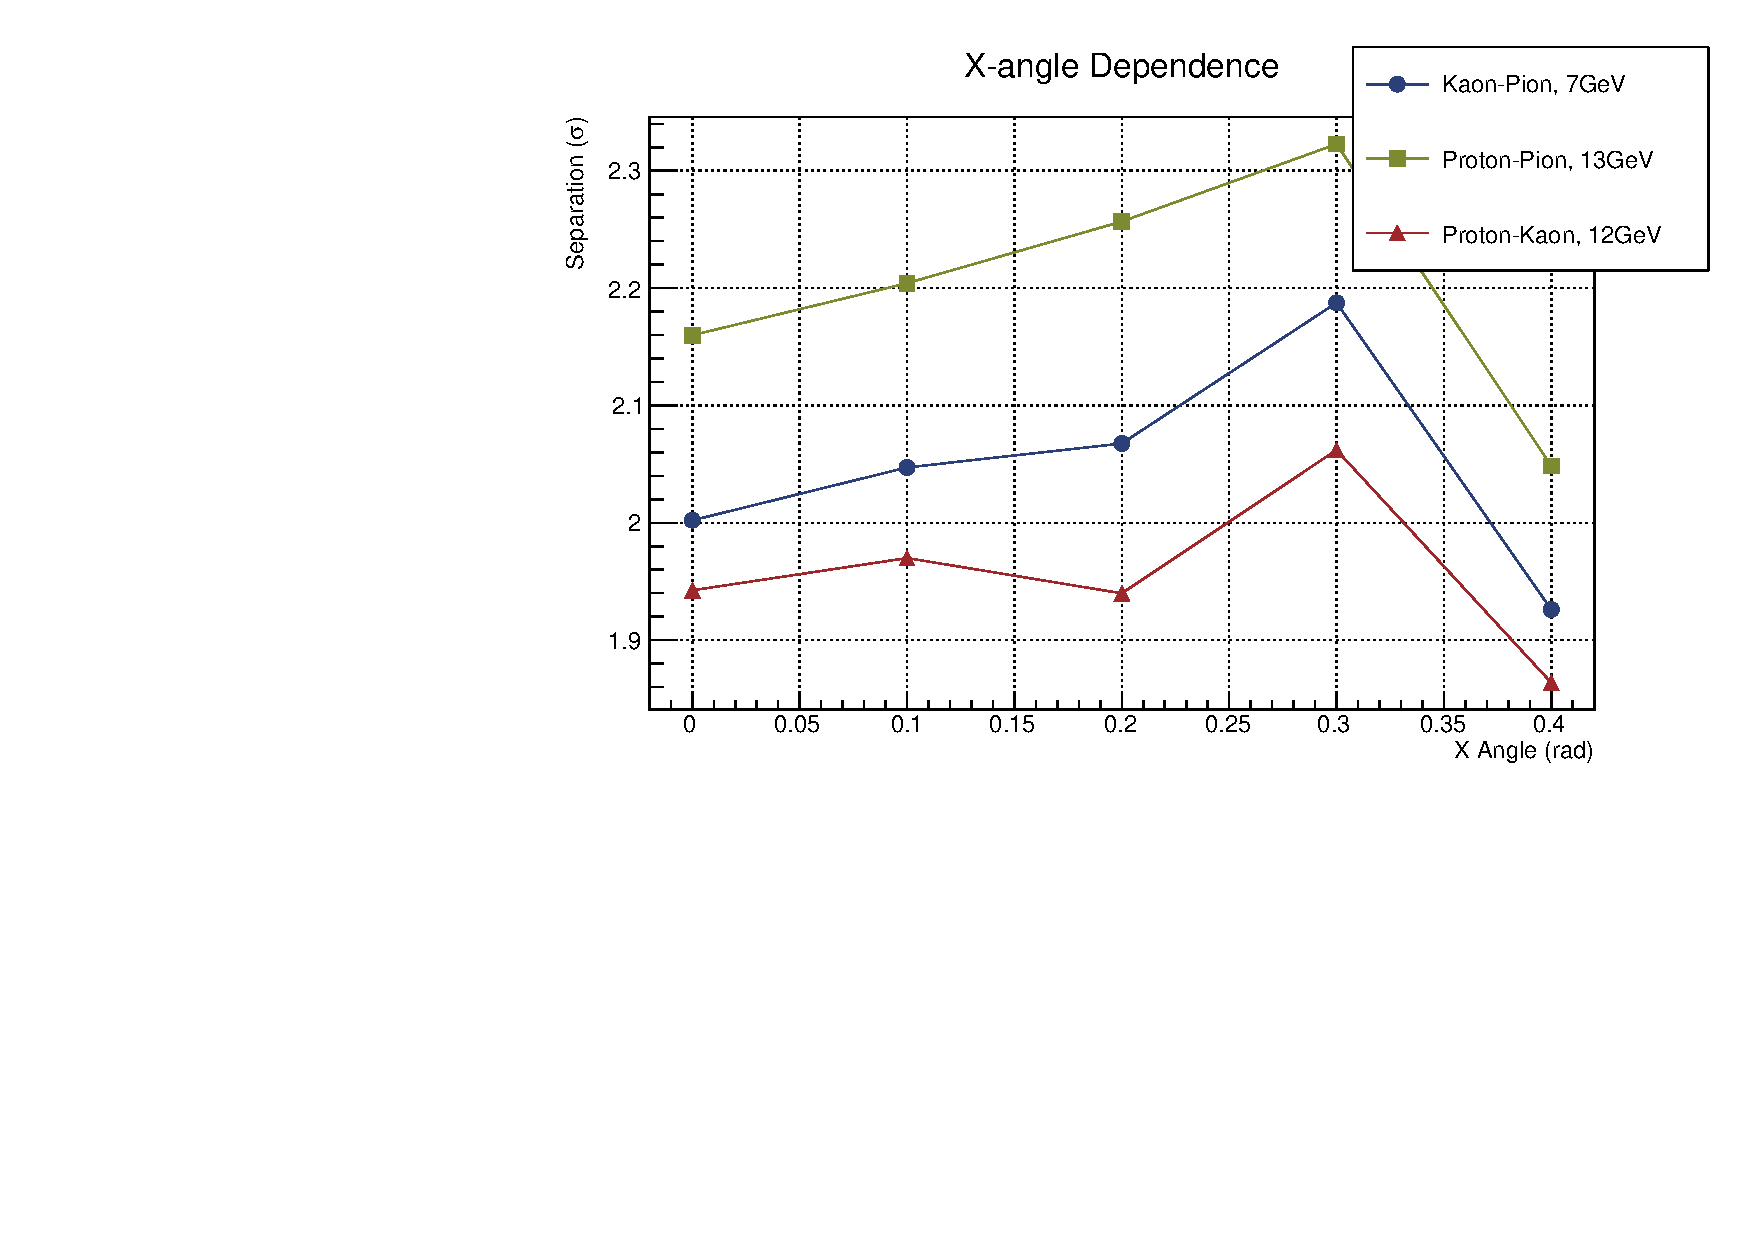
\includegraphics{./figs/xAngleSeps.pdf}}
\caption[\TODO{}]{\TODO{Caption}}
\label{fig:angleSeps}
\end{figure}

\section{Multi-particle events}
Although so far only single-photon ring events have been evaluated, it is often the case that the photons from several different particles will be detected at the same time in the ARICH detector.
It is necessary that the likelihood particle identification technique is able to separate out multi-particle events as well. 

To do this, the simulation was modified to take in a vector of different particle momenta, positions, and directions, rather than just one set of parameters.
Because the photon rings from each particle may overlap with one another and cannot necessarily be disentangled, every possible combination of particle hypotheses must be simulated and compared to the event data in order to concurrently fit all particles.
Because the photon probability distribution functions for each particle are independent, each particle is independently simulated for each particle hypothesis, and the resulting photon histograms are saved.
Next, for every possible combination of these particle hypotheses, we sum together the corresponding particle photon distribution histograms and calculate a log-likelihood by comparing the sum to the event data.
In total, for $n$ detected particles and $p$ possible particle hypotheses, we must simulate $p \times n$ photon distribution functions, do $p^n$  log-likelihood comparisons with our event data, and select the combination with the minimum negative log-likelihood from these $p^n$ options. 

This process is done here: \TODO{Include here the result of running my script to fit multi-particle events, but actually write down the log-likelihoods I get. Also, include figure showing generated multi-particle event, overlayed on the corresponding ``true" photon distribution }.

This particular example was created using random throws of 3 particles with momenta drawn from a Gaussian with mean $\mu$ and standard deviation $\sigma$, and with directions thrown from a Gaussian with mean $\mu$ and standard deviation $\sigma$, a choice of inputs that is entirely arbitrary. \TODO{Include the actual values of $\mu$ and $\sigma$}
In order to get a useful measure of our ability to measure multi-particle events, it is necessary that we better understand what these events might look like in a real experiment.

To find out what these multi-particle events may look like, a simple Geant4 simulation of EMPHATIC was used.
As an example of a typical experimental result, a beam of 10,000 protons with a momentum of 30 GeV/c was simulated.
The protons were generated directly upstream of a 5.0 cm $\times$ 5.0 cm, 2.0 cm thick carbon target, and were directed along the $z$-axis of the experiment.
Geant4 libraries were included to account for elastic scattering, particle decays, hadron physics, stopping physics, and Cherenkov radiation, among other processes. 
The output of the simulation contains information about the identities and trajectories of the particles involved. 
Of interest to this project are specifically the instances where a secondary charged particle enters the aerogel at a velocity sufficient to produce Cherenkov photons.

\TODO{Include matrices of what particles we find as the highest-momentum particles vs. second-highest momentum particle. Key points: The most typical particle-particle combinations are higher-momenta protons with lower-momenta pions, or two pions.} 

It was found that out of the 10,000 events simulated, 24 contained positively charged Kaons entering the aerogel.
\TODO{If I have some time I'll look into the Kaon events.}

\endinput

Any text after an \endinput is ignored.
You could put scraps here or things in progress.
